\documentclass{gdl}

% CHANGE THESE
\def\groupid{BEK}
\def\projectid{AP-GCN}

\usepackage{subcaption}
\usepackage{float}
\usepackage{tikz}

\DeclareMathOperator*{\argmin}{arg\,min}

\graphicspath{{figures/}}

\begin{document}

% CHANGE THIS
\title{AP-GCN Revisited: Replication and Alternative Approaches for Adaptive Propagation in Graph Neural Networks}

% CHANGE THIS
\author{%
Jonatan Bella, Tobias Erbacher, Jonas Knupp\\
\texttt{\{jonatan.bella, tobias.erbacher, jonas.knupp\}@usi.ch}
\vspace{-1.0cm}
}

\begin{abstract}
In conventional Graph Convolutional Networks (GCNs), each node performs a fixed number of message-passing steps. Spinelli et al. proposed Adaptive Propagation GCN (AP-GCN), a model architecture that enables learning an individual number of message-passing steps for each node. This work consists of two main components: a replication study of the AP-GCN paper and an exploration of alternative model architectures that support per-node adaptive message passing.
For the replication study, we re-implemented AP-GCN and evaluated it using the same experimental setup as in the original work. Our results closely matched the accuracies reported by Spinelli et al.
In the second part, we developed three adaptive propagation architectures that adhere to the same constraints as AP-GCN: each node performs at least one message-passing iteration, and once halted, a node remains inactive. The architectures we explored are: RL-AP-GCN, Ponder-AP-GCN (adapted from PonderNet), and Gumbel-AP-GCN (also adapted from PonderNet). Additionally, we evaluated Co-GCN (Cooperative Graph Neural Networks) from Finkelshtein et al., which does not follow the aforementioned constraints.
All four architectures were evaluated under the same conditions as AP-GCN. While our findings show that none of them outperform AP-GCN on any dataset, RL-AP-GCN, Ponder-AP-GCN and Gumbel-AP-GCN achieve competitive results in most of the experiments. 
\vspace{-1.5cm}
\end{abstract}


\maketitle

\section{Introduction}
This work is a replication study of the paper "Adaptive Propagation Graph Convolutional Network" by Indro Spinelli, Simone Scardapane, and Aurelio Uncini \cite{spinelli2021}. In Graph Convolutional Networks (GCNs), each node updates its representation by aggregating and transforming features from its neighbors. This process is repeated over several message passing steps, allowing nodes to incorporate information from increasingly distant parts of the graph. The core contribution of Spinelli et al. is the introduction of the Adaptive Propagation Graph Convolutional Network (AP-GCN) that allows each node in the graph to undergo an individual number of message passing steps. The number of message passing steps per node is learned during training.

In addition to the replication work, we implemented three different model architectures for allowing an individual number of message passing steps per node. The RL-AP-GCN, Ponder-AP-GCN, and Gumbel-AP-GCN model architectures closely follow the constraints and capabilities of the AP-GCN. That is, they do at least one step of message passing and once a node is halted it remains inactive thereafter. Ponder-AP-GCN and Gumbel-AP-GCN are inspired by PonderNet \cite{banino2021}. In addition to these three adaptive propagation model architectures we adopt the cooperative graph convolution network (Co-GCN) architecture from Finkelshtein et al. \cite{finkelshtein2024} to assess whether relaxing the constraints mentioned above improves model performance. We evaluated these four additional model architectures in the same setting as AP-GCN.

We could replicate the findings of Spinelli et al. regarding the accuracy of AP-GCN on all the six datasets. Although our accuracies are marginally lower than those originally reported, the differences are minimal but all outside the 95\% confidence interval. 
Furthermore, while none of our model architectures outperformed AP-GCN, all adaptive propagation architectures achieved reasonable accuracy - in particular considering that we did not have the resources for systematic hyperparameter tuning for each model architecture. Since Co-GCN performed consistently worse than the other adaptive propagation methods in most cases, we conclude that relaxing the constraints did not lead to a better model performance. In addition, we found that Co-GCN is more sensible to the choice of hyperparameters for the given datasets.

The link to our GitHub repository is available in section \ref{sec:experimental-setup}.

\section{Related works}
The main contribution of Spinelli et al. is the introduction of the Adaptive Propagation Graph Convolutional Network (AP-GCN) which enables each node to have an individual number of message passing steps. While Spinelli et al. claim that AP-GCN was at the time the only model in which the number of message passing steps is determined independently for each node and dynamically adjusted during training, there exist model architectures that achieve a similar or at least related goal.

Xu et al. \cite{xu2018} introduced Jumping Knowledge Networks which perform a fixed number of message passes for all nodes and then use per-node LSTM attention to calculate the weighted average over the hidden vectors of the message passing rounds.   

Liu et al. \cite{liu2019} presented GeniePath networks which not only use an attention mechanism to weight the contribution of neighboring nodes but also rely on an LSTM-like gating mechanism that controls the flow of information from one message passing step to the next. In principle, GeniePath networks can learn to stop propagating information individually for each node.

Lai et al. \cite{lai2020} presented Policy-GNN which consists of two modules: a meta-policy module that relies on Deep Q-Learning predicts the required number of message passing steps per node and a GNN module that uses the meta-policy to learn graph representations.

Banino et al. \cite{banino2021} proposed the PonderNet architecture, which dynamically adjusts its computational effort based on the complexity of the given problem. While the authors do not explicitly discuss PonderNet in the context of GNNs, the architecture itself is adaptable to various neural network designs.

Xiao et al. \cite{xiao2021} presented the Learning to Propagate (L2P) framework. They use a latent discrete variable for each node that represents its optimal number of message passing steps. These variables are learned using variational Expectation-Maximization.

Finkelshtein et al. \cite{finkelshtein2024} introduced Cooperative Graph Neural Networks (Co-GNNs) where nodes are in one of the states Standard, Listen, Broadcast, or Isolate. The message-passing behavior of each node is governed by its current state. Nodes in the Broadcast state do not receive any messages but can still send messages — a situation similar to the halting mechanism in AP-GCN.

\section{Methodology}
In this section we first introduce the problem of having an individual number of message passing steps per node. Then, we describe the AP-GCN by Spinelli et al. Lastly, we introduce alternative architectures that allow each node to dynamically adjust its number of message passing steps. In accordance with AP-GCN, we designed all adaptive propagation variants to always do at least one step of message passing per node.

In traditional message-passing graph neural networks, the number of propagation steps is identical for all nodes in the graph. This uniformity implies that each node aggregates information from its neighbors through a fixed number of iterations, regardless of its individual characteristics or position within the graph structure. Spinelli et al. focus on the case where the message-passing is implemented by a Graph Convolution Network (GCN) \cite{kipf2017}. The embedding for node $\mathbf{z}_i$ after $k$ message passing iterations is
\begin{equation}
\mathbf{z}_i^{k} = \sum_{j \in \mathcal{N}(i) \cup \{i\}} \frac{1}{\sqrt{\deg(i)} \cdot \sqrt{\deg(j)}} \left( \mathbf{W}^\top \cdot \mathbf{z}_j^{k-1} \right) + \mathbf{b}
\end{equation}

\subsection{AP-GCN}
The proposed Adaptive Propagation GCN (AP-GCN) enables each node in the graph to perform a distinct number of message-passing iterations, with the number being learned during training rather than set in advance. AP-GCN is inspired by the adaptive computation time in RNNs \cite{graves2017}.

A classifier is added to each node that predicts based on the hidden embedding of a node after $k$ message passing steps whether the propagation should stop. That is, the classifier predicts whether a node should stop aggregating information from its neighbors after $k$ message passing steps. The output of the classifier, $h^k_i$, is the probability the propagation should stop for node $i$ after having performed $k$ steps of message passing.

\begin{equation}
h^k_i = \sigma(\textbf{Q}\textbf{z}^k_i + q)
\end{equation}

\noindent $\textbf{Q}$ and $q$ are trainable parameters and are shared between all nodes. There are two ways the propagation can stop. Firstly, the propagation stops if the number of propagations reaches a predefined maximum number of allowed steps $T$. Secondly, the propagation stops when the propagation budget has been used up. The budget is defined as $1-\epsilon$ where $\epsilon$ is a hyperparameter set to a small value. When $k=K_i$ the budget for node $i$ has been reached after $k$ iterations and the propagation stops. 

\begin{equation}
    K_i = \argmin_{k} \sum_{k=1}^{k} h_i^k \geq 1-\epsilon
\end{equation}

\noindent According to Spinelli et al. the halting probabilities can be combined as

\begin{equation}
    p_i^k = 
    \begin{cases}
    R_i = 1 - \sum_{k=1}^{K_i - 1} h_i^k & \text{if } k = K_i \text{ or } k = T \\
    \sum_{l=1}^{k} h_i^l & \text{otherwise}
    \end{cases}
    \label{eq:p}
\end{equation}

\noindent so that the sequence $\{p_i\}$ forms a \textbf{cumulative probability distribution} (CDF) for the halting probabilities $\{h_i\}$. However, the sequence $\{p_i\}$ does not constitute a CDF, because for $\{p_i\}$ to be a valid CDF, it must satisfy the condition $p_i^k = 1$ when $k = K_i$ or $k = T$. This requirement arises from the fact that a CDF must converge to 1 at its maximum value, reflecting the total probability mass. Clearly, the definition by Spinelli et al., in general, violates this constraint. It could be that the error arose because AP-GCN is inspired by Graves \cite{graves2017} where in equation 6, Graves defines the $\{p_t\}$ to form a \textbf{probability mass function} (PMF) for the $\{h_t\}$ in a similar way. We did not address this issue in the replication code. In the original of \autoref{eq:p} by Spinelli et al. (equation 8) there is a second mistake: they let the sum go from $k=1$ to $K_i$ in the otherwise branch. However, this is just a typo in the paper, in the code they do it as we describe it in \autoref{eq:p}.
The output of the AP-GCN message passing layer for node $i$ is $\hat{\bf{z}}_i$ which is defined as

\begin{equation}
\hat{\mathbf{z}}_i = \frac{1}{K_i} \sum_{k=1}^{K_i} p_i^k \mathbf{z}^k_i + (1-p^k_i) \mathbf{z}_i^{k-1} 
\label{eq:aggregate}
\end{equation}

\noindent Although Spinelli et al. do not state it, this way of accumulating the contribution of the embeddings from the different propagation steps likely is inspired by the soft-conditional output from Scardapane et al. \cite{scardapane2020}.

 The propagation cost $\mathcal{S}_i$ for node $i$ is given by the sum of $K_i$ and $R_i$. Adding $\mathcal{S}_i$ to the loss term incentivizes the model to choose a limited number of propagation steps for node $i$. The propagation penalty $\alpha$ controls the trade-off between accuracy and compute time. A larger $\alpha$ encourages the model to restrict the number of propagation steps per node, whereas a smaller $\alpha$ allows for deeper message passing, potentially improving accuracy at the cost of increased computation. Spinelli et al. decided to update the halting unit once every five epochs. Thus, the final loss is $ \mathcal{\hat{L}} = \mathcal{L} + \alpha \sum_{i\in \mathcal{V}} \mathcal{S}_i $.


\subsection{RL-AP-GCN}
In Graph Neural Networks, node representations tend to homogenize and converge as message passing progresses, a phenomenon known as over-smoothing. Rather than treating this as a limitation, this behavior can serve as a useful signal for an adaptive halting mechanism. Specifically, a reinforcement learning (RL) agent can observe how a node's embedding evolves across propagation steps and learn to halt when changes become minimal, ideally capturing the point of maximum expressiveness for that node. This stabilization suggests diminishing returns from additional message passing, indicating that sufficient neighborhood information has already been integrated. By relying solely on the task reward (e.g., classification accuracy), the policy network can learn to stop propagation at this convergence point, without requiring explicit regularization terms or penalties tied to the number of steps. In doing so, the halting decision becomes a function of information saturation rather than an externally imposed computational constraint.

This reinforcement learning implementation treats each node as an Actor Critic agent but policy and value networks are shared among all nodes. We first compute the initial node embeddings. Then, a loop begins where, at each step, the shared policy network (Actor) evaluates the current embedding of active nodes to output a halting probability, while a shared value network (Critic) estimates the expected future reward (baseline) from that state. A halting action is sampled (incorporating exploration noise during training), and propagation continues for non-halted nodes. Upon halting (or reaching the maximum iterations), a reward is calculated based primarily on the final classification correctness, and the system learns by back propagating a combined loss: a supervised loss for the GNN's classification output, and an RL loss comprising a policy gradient term (using the advantage calculated as actual reward minus the Critic's baseline), a value function loss for the Critic, and an entropy bonus to encourage exploration. To be more precise, I proceed to describe the corresponding operations: 

\paragraph{Halting policy.}
Let $\mathbf{z}_i^{k}\in\mathbb{R}^h$ be the embedding of node $i$ after $k$ message‑passing iterations. At every step the policy network produces the halting probability:
\begin{equation}
\pi_i^{k}=\sigma\bigl(g{\theta}(\mathbf{z}_i^{k})\bigr)
\end{equation}
where the parameters $\theta$ are shared across all nodes. In addition, exploration noise, with the corresponding exploration factor hyperparameter, it is injected by perturbing $\pi_i^{k}$ with Gaussian noise that decays exponentially with the epoch number.This means that even if the policy network is fairly certain a node should continue propagating, the added noise might, for example, push noise high enough for the node to halt, and vice-versa; resulting in a broader exploration of halting points. A Bernoulli action is sampled
\begin{equation}
a_i^{k} \sim \operatorname{Bernoulli}(\pi_i^{k}) ,
\end{equation}
with $a_i^{k}=1$ meaning \emph{halt}. Propagation for node $i$ stops at the first step such that:
\begin{equation}
K_i = \min\{ k \le T \mid a_i^k = 1 \},
\end{equation}
where $T$ is a hard cap on the number of iterations.

\paragraph{Reward and advantage.}
After halting, node $i$ receives a reward:
\begin{equation}
r_i = \mathbb{I}[\hat{y}i = y_i] - cK_i ,
\end{equation}
where $c\ge 0$ is the computation penalty coefficient - that we actually set to 0 during our experiments for the previously explained reasons. A shared value network $V_{\phi}$ provides a baseline, and the resulting advantage is
\begin{equation}
A_i = r_i - V_{\phi}(\mathbf{z}_i^{K_i}).
\end{equation}

\paragraph{Loss function.}
Denote by $\mathcal{V}$ the set of training nodes. The overall objective $\mathcal{V}$ to be minimized combines a standard supervised term (plus L2 regularization $\mathcal{L}_{\text{reg}}$ applied separately) and three reinforcement‑learning components, averaged over the training nodes:
\begin{align}
\mathcal{L} = &\left( \frac{1}{|\mathcal{V}|} \sum_{i\in\mathcal{V}} \mathcal{L}_{\text{NLL}}(y_i, \hat{y}_i) \right) + \mathcal{L}_{\text{reg}} \label{eq:supervised_loss_corr}\\
 &- \frac{1}{|\mathcal{V}|} \sum_{i\in\mathcal{V}} \log\pi_{i}^{K_i} A_i^{\text{detach}} \label{eq:policy_loss_corr}\\
 &+ \lambda_v \frac{1}{|\mathcal{V}|} \sum_{i\in\mathcal{V}} \bigl(r_i - V_{\phi}(\mathbf{z}_i^{K_i})\bigr)^2 \label{eq:value_loss_corr}\\
 &- \lambda_e \frac{1}{|\mathcal{V}|} \sum_{i\in\mathcal{V}} H(\pi_i^{K_i}) \label{eq:entropy_loss_corr}
\end{align}
with $H(p)= -\bigl[p\log p + (1-p)\log(1-p)\bigr]$ the binary entropy. Here $\mathcal{L}_{\text{NLL}}(y_i, \hat{y}_i)$ is the Negative Log-Likelihood loss for node $i$, and $\mathcal{L}_{\text{reg}}$ represents the L2 regularization term (e.g., $\frac{\lambda_{\text{reg}}}{2} \lVert\theta_{\text{reg}}\rVert^2$ applied to specific parameters $\theta_{\text{reg}}$). $A_i^{\text{detach}}$ represents the advantage $r_i - V_{\phi}(\mathbf{z}_i^{K_i})$ where the gradient is not propagated back through the value function estimate $V_{\phi}(\mathbf{z}_i^{K_i})$ during the policy update (as indicated by `detach` - to ensure stable training by preventing the policy update from interfering with the value function update, as the policy might try to manipulate the value estimates to make its own actions look better, rather than simply improving the policy based on the current value estimate.). Hyper‑parameters $\lambda_v$ (corresponding to `value\_weight` in the code) and $\lambda_e$ (corresponding to `entropy\_weight`) weight the value‑regression and entropy‑regularization terms, respectively. The signs reflect the objective minimization: the negative sign in eq.~\eqref{eq:policy_loss_corr} implements policy gradient ascent (maximizing expected rewards), and the negative sign in eq.~\eqref{eq:entropy_loss_corr} encourages entropy maximization (promoting exploration).
    
There are several extensions that could enhance the implementation. The sparse, delayed reward signal could be augmented with denser, intermediate rewards reflecting confidence gains at each step. The RL state representation could be enriched beyond the current embedding to include neighboring node embeddings difference or a history of embeddings (using RNNs or attention), giving the policy more context. Employing more advanced RL algorithms such as PPO for policy updates or GAE for advantage estimation could improve training stability and sample efficiency compared to the current REINFORCE-with-baseline approach. Finally, refining the training strategy, perhaps by alternating between supervised and RL optimization steps, could further stabilize learning and potentially improve final performance.

\subsection{Ponder-AP-GCN}
Strongly inspired by PonderNet \cite{banino2021}, we adopted its core ideas to implement a halting mechanism for GCN. We define $\lambda_i^k$ as the conditional probability that node $i$ halts after $k$ message passing steps given that node $i$ has not halted before. Then, the unconditional probability of node $i$ halting after $k$ message passing iterations is

\begin{equation}
p_i^k = \lambda_i^k \prod_{j=1}^{k-1} (1-\lambda_i^j)
\end{equation}

\noindent which is similar to the geometric distribution but with variable $\lambda$. This would be a valid distribution if we integrated over all possible message passing steps, which is infeasible in practice. For this reason, we define a maximum number of propagation steps $T$ and assign all remaining probability to the last step. This ensures that the $\{p_i^k\}$ for $k\in \{1,...,T\}$ sum to 1. The embedding for node $i$ and therefore implicitly also how many message passing steps are done is then sampled from the random variable $\mathcal{Z}_i$ with probability density distribution $P(\mathcal{Z}_i=\hat{\mathbf{z}}_i^k) = p_i^k$.

The model is trained end-to-end by minimizing the loss function that consists of a sum of two terms weighted by hyperparameter $\beta$: the reconstruction loss and the regularization loss:

\begin{equation}
L = \sum_{i=1}^{\mathcal{|V|}} \sum_{k=1}^{T} \underbrace{p_i^k \mathcal{L}(y_i, \hat{y}_i^k)}_{\text{reconstruction}} + \beta \underbrace{KL(\mathbf{p}_i || p_G(\lambda_p))}_{\text{regularization}}
\label{eq:ponder-loss}
\end{equation}

\noindent where $|V|$ is the number of nodes in the graph.

\noindent The reconstruction loss per node is the cross-entropy loss averaged over the $T$ steps weighted by their corresponding halting probability $p_n$. The regularization term per node incentivizes the distribution $p_n$ to stay close to a predefined prior geometric distribution $p_G$ with parameter $\lambda_p$. In comparison to AP-GCN, this regularization term has the advantage that it is easily interpretable. In particular, setting the prior parameter $\lambda_p = \frac{1}{N}$ encourages the model towards halting after an average of $N$ steps. A disadvantage of Ponder-AP-GCN, compared to AP-GCN, is that during training it must compute the halting distribution over all $T$ steps for each node, whereas AP-GCN can stop computations as soon as a node halts. However, since all the computations in AP-GCN are implemented using matrix operations to deal with all the nodes simultaneously it is questionable whether this is an actual advantage in practice.

Focusing on our implementation, the model architecture starts with an MLP that processes the node features, followed by the recurrent GCN propagation steps - similar to the AP-GCN. A key component is the shared linear halting unit that computes logits at each step, which are passed through a sigmoid function to yield the conditional halting probabilities $\lambda_n$. The unconditional halting distribution $p_n$ is then derived iteratively from these $\lambda_n$  values, ensuring the probabilities sum to one over the maximum N steps. The training loss combines the expected loss (weighted by $p_n$) and the KL divergence between the learned $p_n$ and the geometric prior $p_G$, scaled by $\beta$. Inference can be performed either by first computing the full distribution p and selecting the step via argmax or sampling, or through the computationally efficient sequential Bernoulli sampling at each step as proposed in the PonderNet paper. We implemented the first approach and use the temperature parameter to control the randomness in the model's output. A low temperature makes the model more likely to select high-probability halting steps from $\mathbf{p}_i$, whereas a high temperature increases the likelihood of selecting lower-probability halting steps.

\subsection{Gumbel-AP-GCN}
The Gumbel-AP-GCN architecture is based on the Ponder-AP-GCN architecture but instead of calculating the loss as expectation over the halting steps as in \autoref{eq:ponder-loss}, a halting step $h_i$ for node $i$ is sampled from the learned distribution $\mathbf{p}_i$ of halting steps. We use the Gumbel-Softmax technique \cite{Maddison2017, Jang2017} to draw a sample in a differentiable way. Thus, the halting step for node $i$ is defined as

\begin{equation}
    h_i = \arg\max \text{GumbelSoftmax}(\{\log p_i^1,...,\log p_i^{T}\}, \tau)
\end{equation}

\noindent Where $\tau$ is the temperature parameter controlling how sharp (low $\tau$) or smooth (high $\tau$) the output distribution is. We apply temperature annealing by starting with a higher temperature $\tau_{\text{initial}}$ to encourage a uniform exploration in the early stages of training. $\tau_{\text{warmup}}$ defines the number of epochs during which the temperature is kept constant at $\tau_{\text{initial}}$. Gradually it is lowered to produce less uniform distributions as training progresses - $\tau_{\text{decay}}$ specifies then the number of epochs over which the temperature is linearly annealed from $\tau_{\text{initial}}$ to its $\tau_{\text{final}}$.
Therefore, $\tau$ = $\tau_{\text{initial}}$ during \textit{warmup} period, $\tau$ = $\tau_{\text{final}}$ after \textit{warmup} and \textit{decay}, and as formulated below in the middle of both phases:

\begin{equation}
\tau = \tau_{\text{initial}} - \frac{\text{epoch} - \tau_{\text{warmup}}}{\tau_{\text{decay}}}  * (\tau_{\text{initial}} - \tau_{\text{final}})
\end{equation}

Instead of computing the expected loss over all halting steps like in Ponder-AP-GCN, we compute it from the output corresponding to the sampled step:

\begin{equation}
L = \sum_{i=1}^{\mathcal{|V|}} \underbrace{p_i^{h_i} \mathcal{L}(y_i, \hat{y}_i^{h_i})}_{\text{reconstruction}} + \beta \underbrace{KL(\mathbf{p}_i || p_G(\lambda_p))}_{\text{regularization}}
\end{equation}

\noindent The KL divergence hyperparameter is set to 0, so that the halting policy is learned solely by optimizing the task performance at the sampled steps without explicit regularization. 

The inference is implemented similar to the training. A halting step is sampled using the GumbelSoftmax function and the output corresponding to that halting steps is returned. As in the Ponder-AP-GCN, the inference could be implemented more efficiently using sequential Bernoulli sampling.

\subsection{Co-GCN}
The Cooperative Neural Network (Co-GNN) \cite{finkelshtein2024} architecture is different from the other previously mentioned architectures in the way that we allow a different type of flexibility in Message Passing. In particular, we train a policy that decides which state to assign to a node --- \textsc{Standard}, \textsc{Broadcast}, \textsc{Listen}, or \textsc{Isolate}. These states can be reassigned at each message passing step, so a state that previously was in \textsc{Isolate} could become \textsc{Standard} for the next message passing step, and all combinations thereof. In a sense, the action network modifies the graph in each step, where undirected edges may become directed or simply nonexistent, see \autoref{fig:cognn-actions}.

\begin{figure}[h!]
    \centering
    \begin{tikzpicture}[scale=0.5]
    \node (A) at (- 5 , 1.5) {\small$G$};
    \node (U) at (-6.5, 0) [circle, draw, color=black, minimum size=15pt] {\tiny$u$};
    \node (V) at (- 5 , 0) [circle, draw, color=black, minimum size=15pt] {\tiny$v$};
    \node (W) at (-3.5, 0) [circle, draw, color=black, minimum size=15pt] {\tiny$w$};

    \draw (U) edge[-] (V);
    \draw (V) edge[-] (W);

    %-----

    \node (AA) at (   0, 1.5) {\small$G^{(0)}$};
    \node (BB) at (   0, 1) {\tiny$\{u=I, v=S, w=S\}$};
    \node (UU) at (-1.5, 0) [circle, draw, color=black, minimum size=15pt] {\tiny$u$};
    \node (VV) at (   0, 0) [circle, draw, color=black, minimum size=15pt] {\tiny$v$};
    \node (WW) at ( 1.5, 0) [circle, draw, color=black, minimum size=15pt] {\tiny$w$};

    \draw (VV) edge[<->] (WW);

    %-----

    \node (AAA) at (  5 , 1.5) {\small$G^{(1)}$};
    \node (BBB) at (  5 , 1) {\tiny$\{u=L, v=S, w=B\}$};
    \node (UUU) at ( 3.5, 0) [circle, draw, color=black, minimum size=15pt] {\tiny$u$};
    \node (VVV) at (  5 , 0) [circle, draw, color=black, minimum size=15pt] {\tiny$v$};
    \node (WWW) at ( 6.5, 0) [circle, draw, color=black, minimum size=15pt] {\tiny$w$};

    \draw (UUU) edge[<-] (VVV);
    \draw (VVV) edge[<-] (WWW);
    \end{tikzpicture}
    \captionsetup{justification=centerlast}
    \caption{A graph $G$ and the states $s \in \{S, B, L, I\}$ potentially assigned by a policy at different message passing layers.}
    \label{fig:cognn-actions} 
\end{figure}

A benefit of the dynamically changing graph structure in each layer is that the policy can adjust how to propagate the information at each layer, i.e. for long range tasks it may enable edges while in short range tasks it may isolate most edges for the final propagation layers. Moreover, the authors argue that due the variance introduced by the Co-GNN's stochastic sampling process from the learned policy, this approach can discriminate nodes which are 1-WL (Weisfeiler-Lehman) indistinguishable.

Note that in contrast to the other AP-techniques, the number of propagation is fixed in Co-GNN via the number of layers that the environment network is composed of, however it can still work in a similar manner if the action network were to choose to isolate a node in all successive layers.

In addition, the Co-GNN approach is quite modular since we are able to choose various different architectures for the action and environment networks. In our case, to make the experiments more comparable we will restrain ourselves to use only a CGN architecture, but it is entirely feasible to use GNNs, GATs \cite{veličković2018graphattentionnetworks}, GINs \cite{xu2019powerfulgraphneuralnetworks} etc. as well. For this reason we denote this architecture as Co-GCN instead of Co-GNN.

Regarding the datasets, the ones for node-classification used by the authors are comparable in terms of the statistics described in \autoref{tab:dataset_statistics}, except for the average degree per node, which they do not specify as this is very dependent on what the action network samples, and the homophily ratio which is obviously much different for the heterophilic datasets that they train on.

\section{Implementation}
We independently implemented AP-GCN and compared our implementation with the reference code provided by Spinelli et al., available on their GitHub repository\footnote{\url{https://github.com/spindro/AP-GCN}}. We found that in cases where nodes reach the maximum propagation limit $T$ and are eligible to propagate further, the implementation by Spinelli et al. incorrectly reports one additional step, resulting in an off-by-one error. Importantly, the implementation does not actually perform an extra propagation step—it only misreports the number of steps taken.

For the loading of the Citeseer, Cora-ML, PubMed, MS-Academic, A. Computer, and A. Photo datasets we used the code provided by Spinelli et al.

We asked Prof. Spinelli, among other questions, why they placed the feature mapping layer that projects to the number of classes before the message passing layer. However, we did not receive a response to our email.

\subsection{Datasets}
We downloaded the Citeseer \cite{sen2008}, Cora-ML \cite{mccallum2000}, PubMed \cite{namata2012}, MS-Academic \cite{shchur2018}, A. Computer, and A. Photo datasets from the GitHub repository of Spinelli et al. along with the code to load and process them. The A. Computer and A. Photo datasets are portions of the Amazon co-purchase graph originally presented in \cite{mcauley2015}. In the MS-Academic dataset, the edges represent co-authorship while in the Citeseer, Cora-ML, and PubMed datasets, the edges represent citations. All these datasets consists of a single graph and are node classification problems. Only the largest connected component in each dataset is used. We calculated the statistics for each dataset, as shown in \autoref{tab:dataset_statistics}. Except for a few values in the average degrees, which may be due to rounding, our results are consistent with those reported by Spinelli et al. Note that the homophily ratio was not reported by Spinelli et al. All the graphs are quite strongly homophilic.

\begin{table}[h]
    \footnotesize\sf
    \setlength{\tabcolsep}{1pt}
    \caption{Dataset Statistics}
    \begin{tabular}{l c c c c c c}
        \toprule
        Dataset & Classes & Features & Nodes & Edges & Avg. Degr. & Homo. Ratio \\
        \midrule
        Citeseer & 6 & 3703 & 2110 & 3668 & 6.95 & 0.74 \\
        Cora-ML & 7 & 2879 & 2810 & 7981 & 11.36 & 0.78 \\
        PubMed & 3 & 500 & 19717 &44324 &8.99 & 0.80 \\
        MS-Academic & 15&6805 & 18333 & 81894 & 17.87 & 0.81 \\
        A.Computer & 10 & 767 & 13381 & 245778 & 73.47 & 0.78 \\
        A.Photo  & 8 & 745 & 7487 & 119043 & 63.60 & 0.83 \\
        \bottomrule
    \end{tabular}
    \label{tab:dataset_statistics}
\end{table}

\subsection{Hyperparameters}
In the experiments with AP-GCN we used the hyperparameters described in the paper by Spinelli et al. They are described in appendix \ref{lab:hyper-ap-gcn}. The hyperparameters used in the experiments with RL-AP-GCN, Ponder-AP-GCN, Gumbel-AP-GCN, and Co-GCN are available in appendices \ref{lab:hyper-rl-gcn}, \ref{lab:hyper-ponder-gcn}, \ref{lab:hyper-gumbel-gcn}, and \ref{lab:hyper-Co-GCN}. We did not perform systematic hyperparameter optimization for RL-AP-GCN, Ponder-AP-GCN, Gumbel-AP-GCN, and Co-GCN. Instead, we mostly tested each model on the Cora-ML dataset and once we obtained reasonably good hyperparameters we reused them for the other datasets. 

\subsection{Experimental setup}
\label{sec:experimental-setup}
We follow the experimental setup of Spinelli et al., splitting each dataset into a development and a test set. Spinelli et al. follow the experimental setup of \cite{Klicpera2019}. The test set serves to evaluate the final model performance. The development set is split into the training and validation set. The training set consists of 20 instances per class sampled from the development set. The rest of the development set is assigned to the validation set which is used for early stopping. For the MS-Academic dataset, the development set consists of 5,000 samples, whereas for all other datasets it contains 1,500 samples. This larger size is chosen for MS-Academic because a smaller development set of 1,500 samples would likely result in fewer than 20 samples per class. 

For each dataset, we use 20 random seeds to sample a training set from the development set, and for each seed, the model is trained five times with different weight initializations, resulting in 100 trained models per dataset for a fixed set of hyperparameters. While Spinelli et al. provided the 20 seeds for the sampling of the training sets, there is still a degree of randomness involved because Spinelli et al. did not provide seeds for the model initializations.

Our code is available on GitHub\footnote{\url{https://github.com/TobiasErbacher/gdl}}.

\subsection{Computational requirements}
The experiments involving the adaptive propagation architectures were carried out on a MacBook Pro equipped with an Apple M2 Pro chip and 16 GB of memory, using the MPS backend in PyTorch. We encountered a peculiar issue with the CoGNN model on this backend: after a certain number of epochs, the loss began to contain NaN (not-a-number) values. Despite trying several potential fixes, the problem persisted. However, when switching to a different backend, either CPU or CUDA, with the same hyperparameters, the issue did not occur. As a result, we opted to run the CoGNN models on machines with an Nvidia GPU. Specifically, experiments on the Amazon datasets were conducted on a machine with a Tesla T4 GPU (16 GB VRAM), while those on all other datasets were run on a GeForce RTX 3050 Ti Laptop (4 GB VRAM). Although the hardware differences make direct comparisons of training time per epoch challenging, all systems used are consumer-grade and relatively similar in capability.

\autoref{tab:total-compute-time} shows the compute time per model architecture and the total compute time. Note that the reported compute times only cover the main experiments described in section \ref{sec:experimental-setup} not the compute time related to debugging the model architectures and the setup of the benchmarking code.

\begin{table}[h]
    \small\sf
    \setlength{\tabcolsep}{2pt}
    \caption{Compute time by model architecture and total compute time.}
    \begin{tabular}{l c c c c c c}
        \toprule
        Model Architecture & Total Compute Time [h]\\
        \midrule
        RL-AP-GCN & 20.23 \\
        Ponder-AP-GCN & 8.77 \\
        Gumbel-AP-GCN & 11.49 \\
        Co-GCN & 8.10   \\
        AP-GCN replication & 7.63  \\
        \midrule
        Total & 56.22 \\
        \bottomrule
    \end{tabular}
    \label{tab:total-compute-time}
\end{table}


\section{Results}
We report the results of our experiments with the AP-GCN, RL-AP-GCN, Ponder-AP-GCN, Gumbel-AP-GCN, and Co-GCN architectures. \autoref{tab:accuracy} shows the average accuracy, with uncertainties showing the 95\% confidence level calculated by bootstrapping. The uncertainty is defined as the larger absolute difference between the mean and the 2.5th or 97.5th percentile of the bootstrap distribution. This follows the code in the Jupyter notebook provided by Spinelli et al. The accuracies of the replicated AP-GCN are consistently lower than the ones reported by Spinelli et al. The largest difference 2.02\% occurs on the Cora-ML dataset. Given that we did not use the exact same setup (library versions and seeds for the model initializations) as Spinelli et al. we think these differences are acceptable. 

In \autoref{fig:density-distribution} we report the distribution of the halting steps, i.e., the steps at which each node halts for the adaptive propagation model architectures. Since we have data from 100 runs per model architecture, we first average the halting steps for each node over the 100 runs and then plot the distribution obtained using kernel density estimation (KDE) over these averaged halting steps per node. Note that because of the averaging and the KDE there can be probability mass at non-integer values even though in reality all the models can only halt at an integer number of steps. This approach follows the methodology used by Spinelli et al. The step distribution for AP-GCN has a spike for the MS-Academic (ca. 2.6) and A.Computer (ca. 3.9) datasets at around 2 steps. All other models do not show such pronounced spikes. Furthermore,  the density distributions of different datasets under AP-GCN differ significantly from those of other model architectures, where the peaks of the distributions are typically closer together. In Gumbel-AP-GCN the densities for all datasets are almost identical and centered around 3.5 @Jonathan what could be problem. An important result is that the datasets do not enforce a certain step distribution independent of the model architecture. The reason for this could be that the optimal number of message passing iterations per node depends on the behavior of the neighboring nodes. Consequently, we suspect that there might exist many good combinations of halting steps for a graph.

\autoref{fig:steps-dist-steps-std} shows the distribution of the standard deviations per node over the 100 experiments for each dataset. A low median standard deviation is desirable since it shows that a model often returns similar halting steps for the same node over experiments with different seeds and weight initialization. Furthermore, it is desirable that the median standard deviation is consistent across the different datasets. AP-GCN tends to have a very low standard deviation per node. RL-AP-GCN has a high standard deviation per node for each dataset. Interestingly, the medians of the boxplots are almost identical (around 3.6). Ponder-AP-GCN has low median standard deviation per node in the Cora-ML, MS-Academic, A.Computer, and A.Photo datasets and high median standard deviation per node in the Citeseer and PubMed datasets. Gumbel-AP-GCN has a high standard deviation per node but still lower than RL-AP-GCN. 

The average training time per epoch for each model is shown in \autoref{tab:time-per-epoch}. While the training times we obtained for AP-GCN differ slightly from those reported by Spinelli et al., this is likely due to differences in hardware; nonetheless, the values remain comparable. Across most datasets, Ponder-AP-GCN is nearly as fast as AP-GCN and even outperforms it on the Cora-ML and PubMed datasets. Unsurprisingly, RL-AP-GCN exhibits the longest training times. @Jonathan, could you elaborate on why this is expected and how it relates to reinforcement learning? Additionally, the variation in training time per epoch across datasets is more pronounced for Co-GCN than for AP-GCN.

Instead of reporting the distribution of halting steps, we tracked how the nodes were distributed among the four possible states at each step. \autoref{fig:cooperative-result} displays boxplots representing the variation in the proportion of nodes assigned to each state (standard, broadcast, listen, and isolate) across 100 independent runs, for each dataset and step. In the experiments on Citeseer, Cora-ML, PubMed, and MS-Academic, the majority of nodes remain in the standard state across nearly all 100 runs and at every step. In contrast, for the A.Computer and A.Photo experiments, nodes tend to be almost evenly distributed across the different states at each step. @Tobias write more about the figure (eg expected that less nodes in standard step because larger avg degree, possible explanation why performance worse for large degree datasets)

\section{Discussion and conclusion}
Although AP-GCN performs well in practice, several of its design choices lack clear theoretical justification in our opinion. For example, Spinelli et al. refer to $h_i^k$ as the probability that a node should halt after $k$ iterations. However, this is not what actually happens in the model: a node halts only when its propagation budget is used up or the maximum number of steps is reached. For instance, assume we have $\mathbf{h}_i = [0.3, 0.4, 0.25]$ and a propagation budget of $0.9$. AP-GCN will not halt node $i$ with probability $0.3$ after the first step. In fact, it will never halt after the first step. It will only halt after the third step, once the budget is fully consumed. Similarly, the way embeddings are aggregated over steps in \autoref{eq:aggregate} lacks a clear theoretical foundation.

We particularly appreciate how seamlessly the PonderNet framework can be adopted to adaptive propagation within graph convolutional networks. Unlike AP-GCN, Ponder-AP-GCN rests on a solid theoretical basis. Although its empirical performance trails AP-GCN slightly, more thorough hyperparameter optimization could possibly allow Ponder-AP-GCN to surpass AP-GCN.

For Co-GCN, future work could explore modifying the architecture to share the environment network across steps, thereby reducing the overall parameter count and harnessing potential synergy effects.

\begin{figure*}[p]
    \centering
    \begin{minipage}[t]{0.48\textwidth}
        \centering
        \begin{subfigure}[b]{0.8\textwidth}
            \centering
            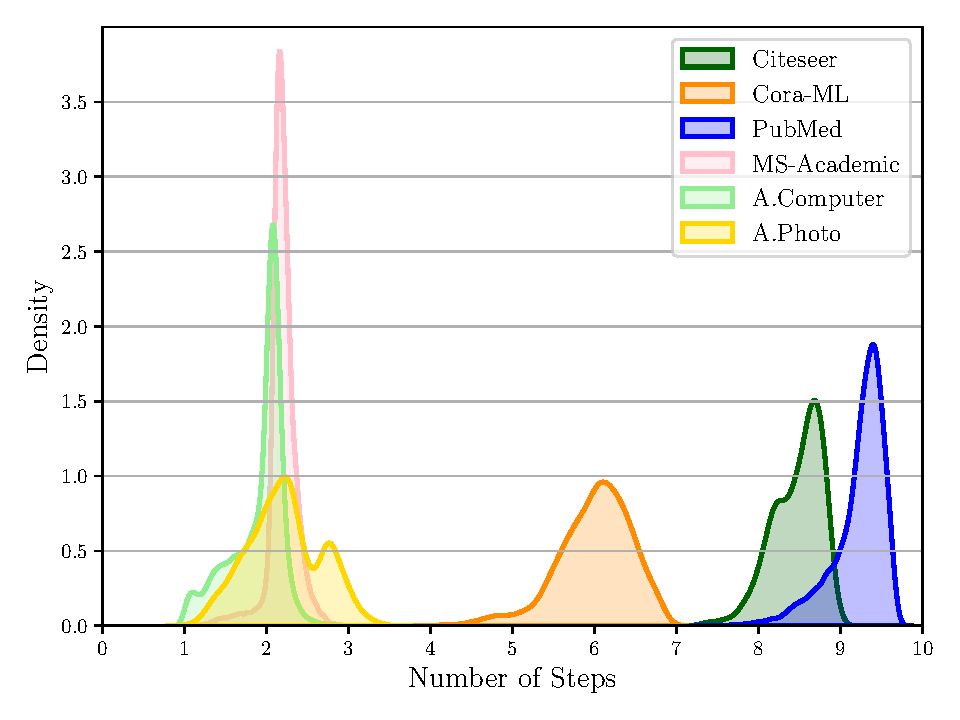
\includegraphics[width=\textwidth]{Spinelli_steps_distribution.pdf}
            \captionsetup{justification=centerlast}
            \caption{AP-GCN Replication}
            \label{fig:step_dist_AP_GCN}
        \end{subfigure}
        
        \begin{subfigure}[b]{0.8\textwidth}
            \centering
            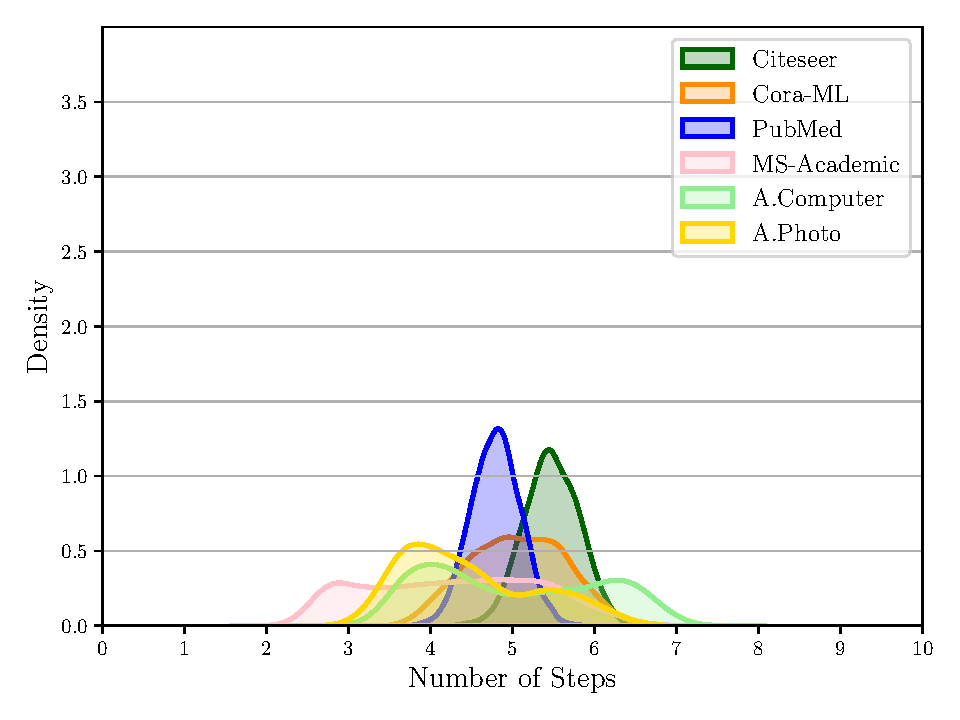
\includegraphics[width=\textwidth]{RL-AP-GCN_steps_distribution.pdf}
            \captionsetup{justification=centerlast}
            \caption{RL-AP-GCN}
            \label{fig:step_dist_RL_AP_GCN}
        \end{subfigure}
        
        \begin{subfigure}[b]{0.8\textwidth}
            \centering
            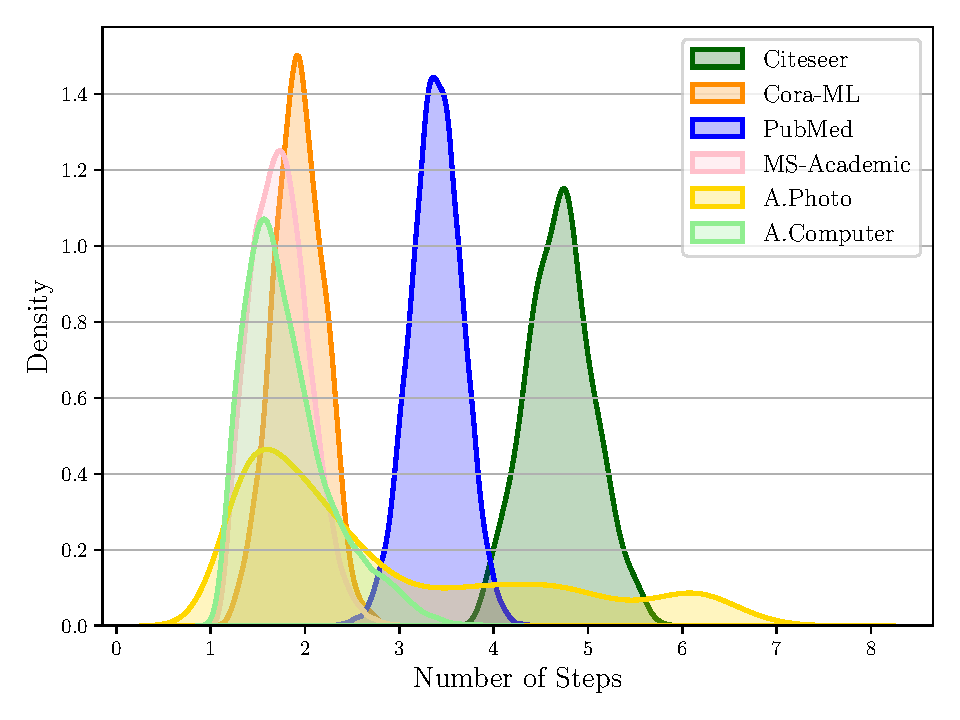
\includegraphics[width=\textwidth]{Ponder-AP-GCN_steps_distribution.pdf}
            \captionsetup{justification=centerlast}
            \caption{Ponder-AP-GCN}
            \label{fig:step_dist_Ponder_AP_GCN}
        \end{subfigure}
        
        \begin{subfigure}[b]{0.8\textwidth}
            \centering
            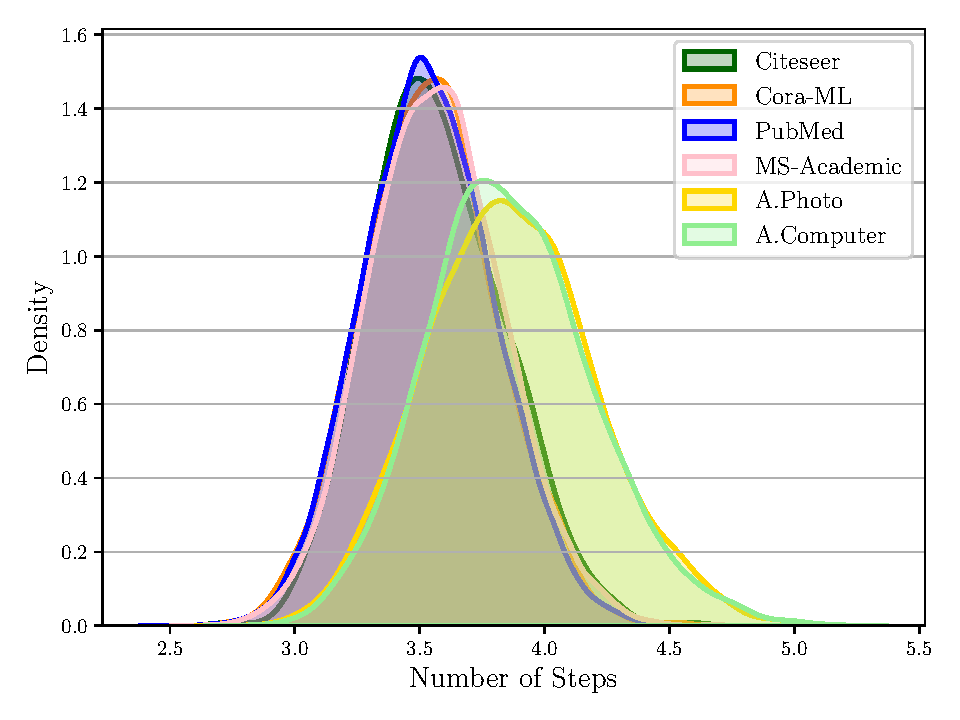
\includegraphics[width=\textwidth]{Gumbel-AP-GCN_steps_distribution.pdf}
            \captionsetup{justification=centerlast}
            \caption{Gumbel-AP-GCN}
            \label{fig:step_dist_Gumbel_AP_GCN}
        \end{subfigure}
        
        \captionsetup{justification=centerlast}
        \caption{Average density distribution of the halting steps for the five different model architectures for each dataset.}
        \label{fig:density-distribution}
    \end{minipage}%
    \hfill
    \begin{minipage}[t]{0.48\textwidth}
        \centering
        \begin{subfigure}[b]{0.8\textwidth}
            \centering
            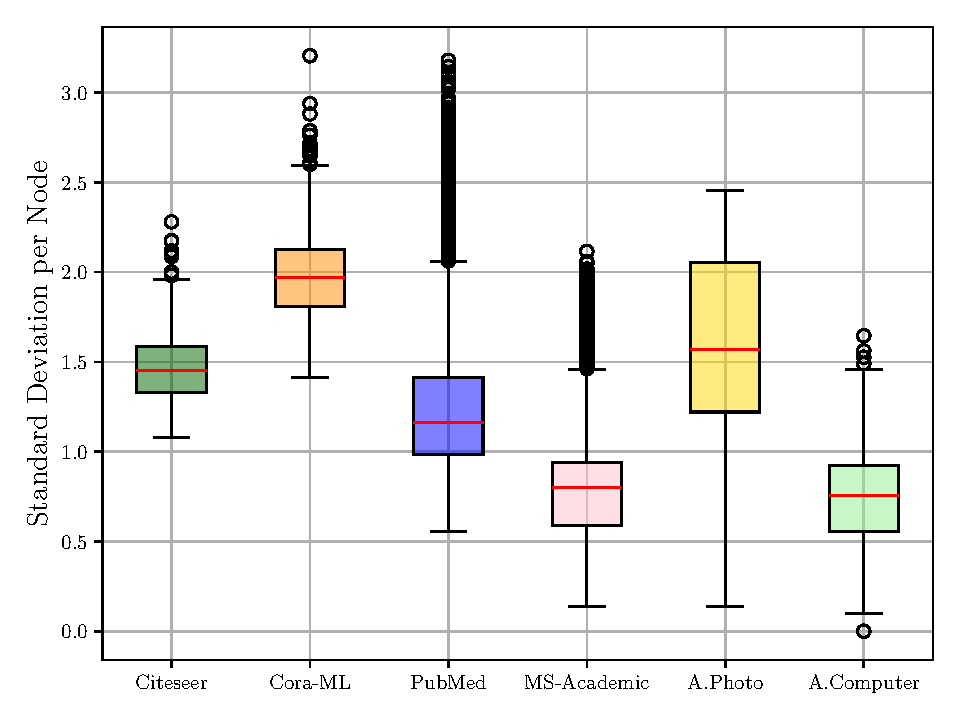
\includegraphics[width=\textwidth]{Spinelli_std_steps_per_node_boxplot.pdf}
            \captionsetup{justification=centerlast}
            \caption{AP-GCN Replication}
            \label{fig:step_std_AP_GCN}
        \end{subfigure}
        
        \begin{subfigure}[b]{0.8\textwidth}
            \centering
            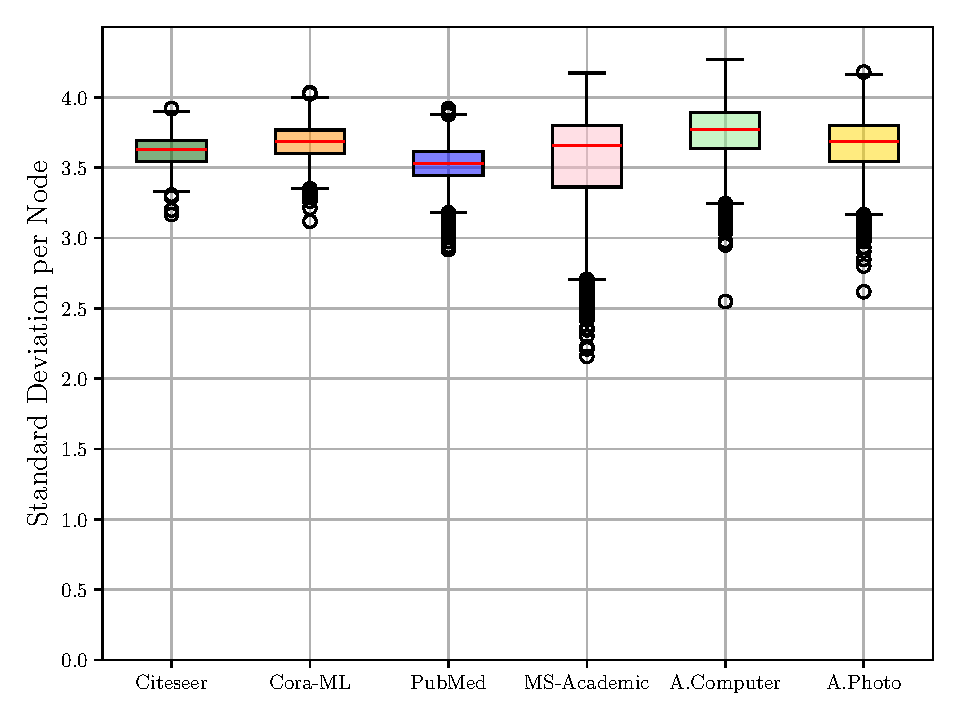
\includegraphics[width=\textwidth]{RL-AP-GCN_std_steps_per_node_boxplot.pdf}
            \captionsetup{justification=centerlast}
            \caption{RL-AP-GCN}
            \label{fig:step_std_RL_AP_GCN}
        \end{subfigure}
        
        \begin{subfigure}[b]{0.8\textwidth}
            \centering
            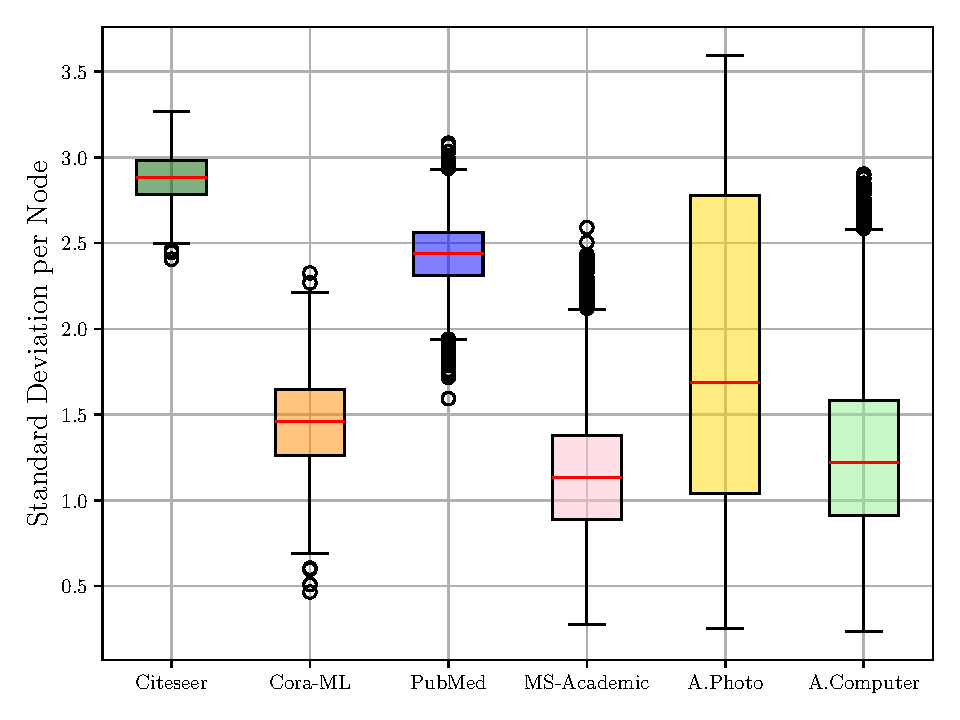
\includegraphics[width=\textwidth]{Ponder-AP-GCN_std_steps_per_node_boxplot.pdf}
            \captionsetup{justification=centerlast}
            \caption{Ponder-AP-GCN}
            \label{fig:step_std_Ponder_AP_GCN}
        \end{subfigure}
        
        \begin{subfigure}[b]{0.8\textwidth}
            \centering
            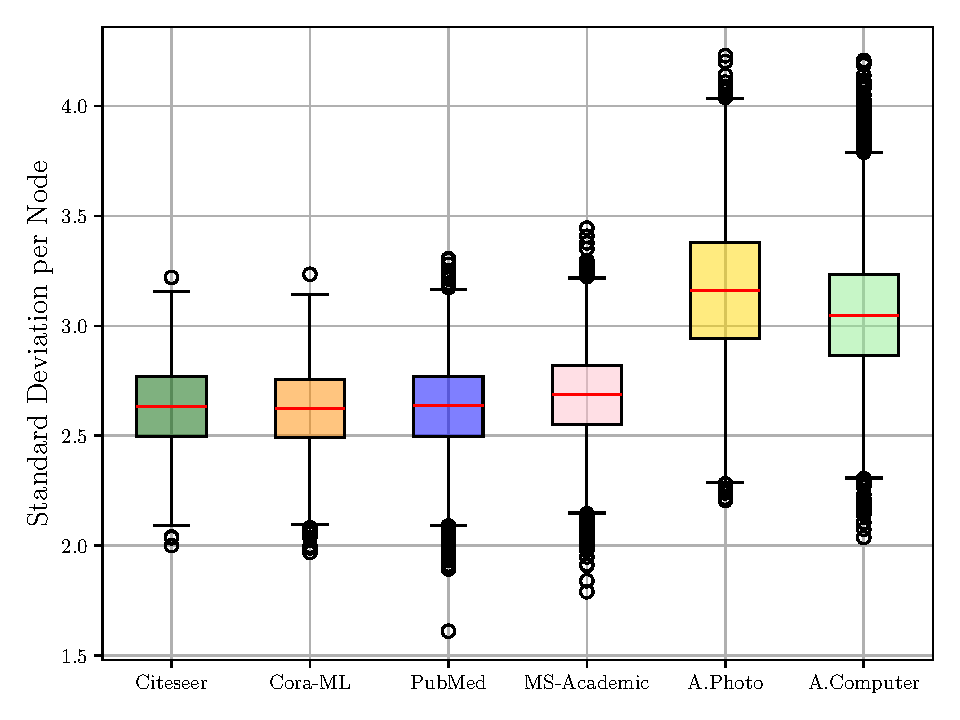
\includegraphics[width=\textwidth]{Gumbel-AP-GCN_std_steps_per_node_boxplot.pdf}
            \captionsetup{justification=centerlast}
            \caption{Gumbel-AP-GCN}
            \label{fig:step_std_Gumbel_AP_GCN}
        \end{subfigure}

        
        \captionsetup{justification=centerlast}
        \caption{Standard deviations per node over the 100 experiments for each dataset.}
        \label{fig:steps-dist-steps-std}
    \end{minipage}
\end{figure*}

\newpage
\onecolumn

\begin{table}[h]
    \small\sf\centering
    \caption{Average test set accuracies with 95\% confidence intervals, computed from 100 runs per model using 20 random seeds and 5 different initial weight settings per seed.}
    \begin{tabular}{l c c c c c c}
        \toprule
        Model & Citeseer & Cora-ML & PubMed & MS-Academic & A.Computer & A.Photo\\
        \midrule
        \texttt{RL-AP-GCN} &$74.66 \pm 0.30$&$81.63 \pm 1.43$&$77.18 \pm 0.44$&$88.32 \pm 0.45$&$79.97 \pm 0.56$&$88.88 \pm 0.40$   \\
        \texttt{Ponder-AP-GCN} &$74.80 \pm 0.33$&$82.14 \pm 0.28$&$76.37 \pm 0.43$&$91.29 \pm 0.12$&$83.41 \pm 0.27$&$91.28 \pm 0.23$  \\
        \texttt{Gumbel-AP-GCN} &$70.12 \pm 1.43$&$70.86 \pm 2.50$&$76.85 \pm 0.41$&$87.56 \pm 0.41$&$79.13 \pm 0.55$&$89.22 \pm 0.39$  \\
        \texttt{Co-GCN} &$68.00 \pm 0.77$&$74.80 \pm 2.14$&$75.89 \pm 1.04$&$88.58 \pm 0.20$&$30.47 \pm 1.16$&$34.42 \pm 3.57$  \\
        \texttt{AP-GCN replication} &$75.87 \pm 0.27$&$83.69 \pm 0.34$&$78.97 \pm 0.41$&$91.65 \pm 0.13$&$83.25 \pm 0.34$&$90.69 \pm 0.32$        \\
        \midrule
        \texttt{AP-GCN} & $76.12 \pm 0.24$ & $85.71 \pm 0.22$ & $79.80 \pm 0.34$ & $92.62 \pm 0.07$ & $85.18 \pm 0.23$ & $92.05 \pm 0.22$\\
        \bottomrule
    \end{tabular}
    \label{tab:accuracy}
\end{table}

\begin{figure}[h]
    \centering 
        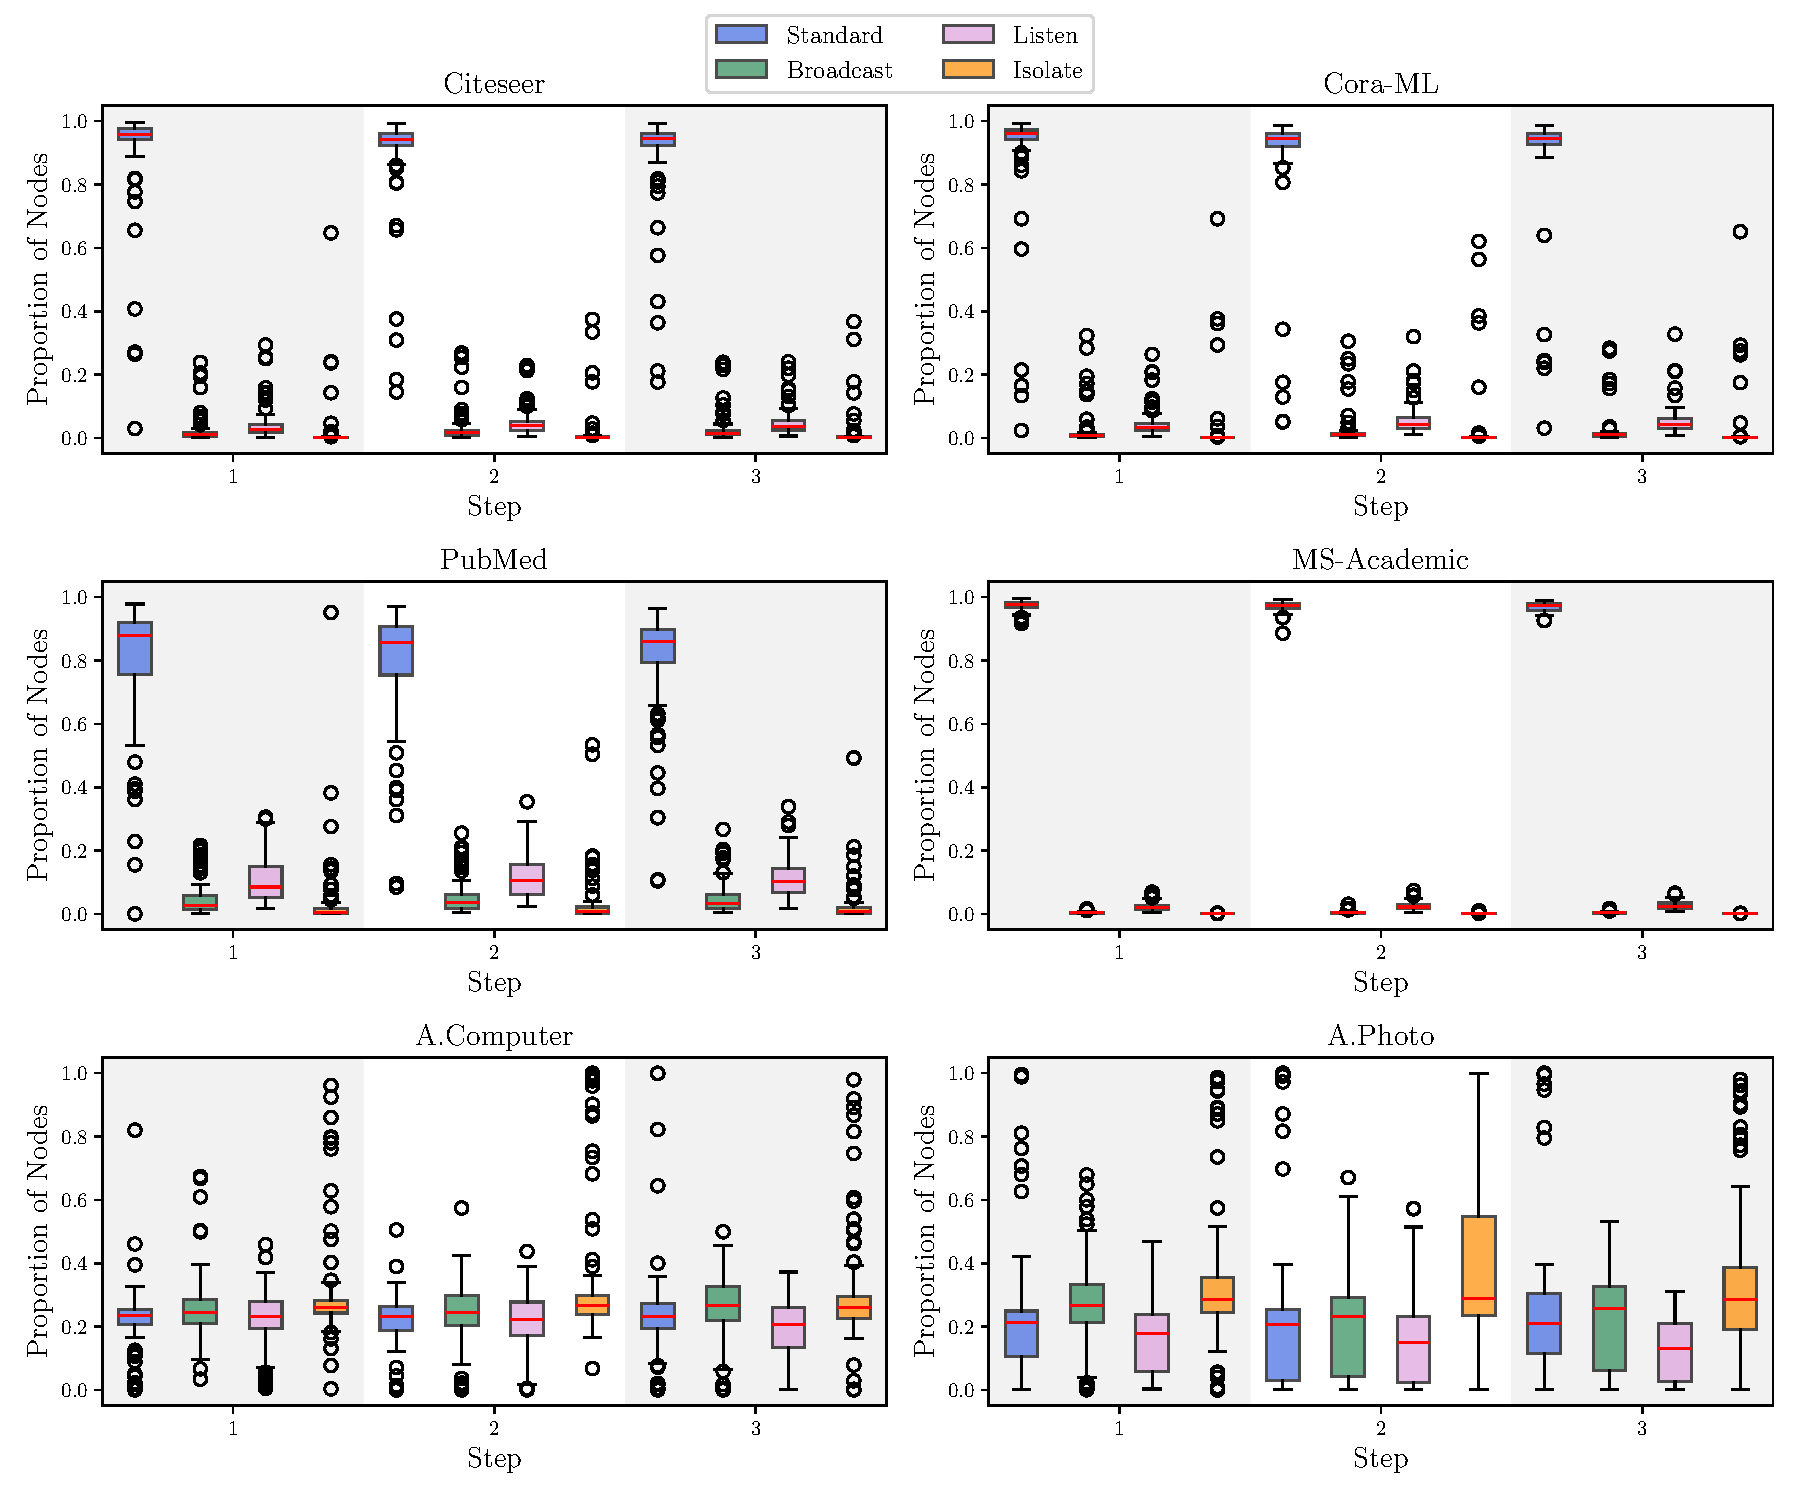
\includegraphics[width=0.9\textwidth]{Cooperative-AP-GCN_state_distribution_per_step.pdf}
        \caption{Each figure shows the distribution of the proportion of nodes in a given state per layer of the Co-GCN models for a dataset.}
        \label{fig:cooperative-result} 
\end{figure}



\begin{table}[h]
    \small\sf\centering
    \caption{Average training time per epoch in milliseconds, computed from 100 runs per model using 20 random seeds and 5 different initial weight settings per seed.}
    \begin{tabular}{l c c c c c c}
        \toprule
        Model & Citeseer & Cora-ML & PubMed & MS-Academic & A.Computer & A.Photo   \\
        \midrule
        \texttt{RL-AP-GCN} &$169.0$&$161.6$&$221.4$&$279.0$&$279.8$&$206.1$  \\
        \texttt{Ponder-AP-GCN} &$54.1$&$51.1$&$67.9$&$136.4$&$173.6$&$87.9$   \\
        \texttt{Gumbel-AP-GCN} &$81.5$&$84.8$&$84.9$&$157.3$&$188.8$&$112.5$   \\
        \texttt{Co-GCN} &$52.4$&$52.4$&$213.5$&$131.6$&$290.4$&$236.0$  \\
        \texttt{AP-GCN replication} &$48.1$&$51.5$&$79.1$&$117.5$&$113.5$&$78.6$  \\
        \midrule
        \texttt{AP-GCN} & $32.4$ & $36.2$ & $42.0$ & $100.3$ & $76.7$ & $50.0$ \\
        \bottomrule 
    \end{tabular}
    \label{tab:time-per-epoch}
\end{table}

\newpage
\twocolumn




\clearpage
% Bibliography
\bibliography{bibliography}
\bibliographystyle{unsrtnat}
\clearpage

\appendix

\section{Hyperparameters}
The maximum number of steps $T$ was set to 10 for all experiments.

\subsection{AP-GCN}
\label{lab:hyper-ap-gcn}
We use 2 feature transformation layers, a dropout rate of 0.5, 64 hidden units, and the Adam optimizer with learning rate 0.01. We applied $L2$ regularization with coefficient 0.008 on the parameters of the first layer. For the \texttt{A. Photo} and \texttt{A. Computer} no regularization was used.

\subsection{RL-AP-GCN}
\label{lab:hyper-rl-gcn}
We used the Adam optimizer with a learning rate of 0.01. The model employs a dropout rate of 0.5 and 64 hidden units. $L_2$ regularization with a coefficient of 0.008 was applied to the parameters of the first layer, except for the \texttt{A. Photo} and \texttt{A. Computer} datasets, where no regularization was used. The entropy weight was set to 0.01, and the value weight to 0.5. Gradient norm clipping was applied across all model parameters with a maximum norm of 1.0. Additionally, we set the computation penalty to 0, used an exploration factor of 0.01, and did not employ any scheduling for the exploration penalty.

\subsection{Ponder-AP-GCN}
\label{lab:hyper-ponder-gcn}
We used the Adam optimizer with a learning rate of 0.01. The model incorporates a dropout rate of 0.5, an edge dropout rate of 0.3, and 64 hidden units. Edge dropout was applied only in the section focused on adaptive message propagation. $L_2$ regularization with a coefficient of 0.008 was applied to the parameters of the first layer, except for the \texttt{A. Photo} and \texttt{A. Computer} datasets, where no regularization was used. We set $\beta$ to 0.01 and $\lambda_p$ to 0.2. During inference, a temperature value of 5.0 was used.

\subsection{Gumbel-AP-GCN}
\label{lab:hyper-gumbel-gcn}
We employed the Adam optimizer with a learning rate of 0.01. The model uses a dropout rate of 0.5, an edge dropout rate of 0.3, and 64 hidden units. Edge dropout was applied exclusively in the adaptive message propagation component. $L_2$ regularization with a coefficient of 0.008 was applied to the parameters of the first layer, except for the \texttt{A. Photo} and \texttt{A. Computer} datasets, where no regularization was used. We set $\beta$ to 0, indicating that the model learns without a geometric prior, rendering $\lambda_p$ irrelevant. During training we use a scheduler for $\tau$ with $\tau_{\text{initial}} = 10.0$, $\tau_{\text{warmup}} = 20.0$, $\tau_{\text{decay}} = 50.0$, and $\tau_{\text{final}} = 1.0$. During evaluation, $\tau$ was fixed at 0.01.

\subsection{Co-GCN}
\label{lab:hyper-Co-GCN}
@Tobias (see bottom of model file in replication folder)

\end{document}
